\section{20 Nov 23 - Notes: Random
Processes}\label{nov-23---notes-random-processes}

Until now, all of our work has been with
\href{https://en.wikipedia.org/wiki/Deterministic_system}{deterministic
systems}. That is, we have a set of equations that allow us to describe
the future of the system in space and time with certainty. Some
differential equations are deterministic and all the ones that we have
worked on so far are. Our analysis of ordinary differential equations,
partial differential equations, and the wave equation have all been
drawn from deterministic systems. We obtain equations or results that we
can predict with (up to numerical) certainty.

However, many processes in nature are not deterministic. These processes
are stochastic, probabilistic, or
\href{https://en.wikipedia.org/wiki/Randomness}{random}. We use these
terms interchangeably, but ultimately the all describe a system with
probabilistic states. These can be things like
\href{https://en.wikipedia.org/wiki/Ideal_gas}{the ideal gas in
statistical mechanics} or
\href{https://en.wikipedia.org/wiki/Hydrogen_atom}{the hydrogen atom in
quantum mechanics}. But this work applies in contexts like the
\href{https://bsj.berkeley.edu/how-scientists-are-using-statistical-physics-to-predict-the-stock-market/}{stock
market},
\href{https://en.wikipedia.org/wiki/Numerical_weather_prediction}{weather},
\href{https://journals.aps.org/pre/abstract/10.1103/PhysRevE.104.014132}{the
spread of disease}, and even
\href{https://en.wikipedia.org/wiki/Information_theory}{information
theory}.

\subsection{Entropy}\label{entropy}

We will start with the concept of
\href{https://en.wikipedia.org/wiki/Entropy}{entropy}, which serves as a
major organizing idea for many statistical physics models and results.
For example, conservation of energy tells us that the same amount of
energy is needed for a ball to change its height (moving up or down),
but the concept of increasing entropy indicates the ball won't
spontaneously jump off the table.

\subsubsection{Video}\label{video}

Later, we will develop a mathematical definition of entropy, when we
introduce \href{https://en.wikipedia.org/wiki/Combinatorics}{counting
statistics}. The result, developed by
\href{https://en.wikipedia.org/wiki/Ludwig_Boltzmann}{Ludwig Boltzmann},
is quoted below:

\[S = k \ln(\Omega)\]

where \(k\) is the
\href{https://en.wikipedia.org/wiki/Boltzmann_constant}{Boltzmann
constant} and \(\Omega\) is the
\href{https://en.wikipedia.org/wiki/Multiplicity_(statistical_mechanics)}{``multiplicity''}
of the system. The video below from
\href{https://www.youtube.com/channel/UCHnyfMqiRRG1u-2MsSQLbXA}{Veritasium}
provides a nice introduction to the concept of entropy.

\href{https://inv.tux.pizza/watch?v=DxL2HoqLbyA}{\pandocbounded{\includegraphics[keepaspectratio,alt={Entropy}]{https://markdown-videos-api.jorgenkh.no/youtube/DxL2HoqLbyA?width=720&height=405}}}

\begin{itemize}
\tightlist
\item
  Non-Commercial Link: \url{https://inv.tux.pizza/watch?v=DxL2HoqLbyA}
\item
  Commercial Link: \url{https://youtube.com/watch?v=DxL2HoqLbyA}
\end{itemize}

\subsection{Modeling Randomness}\label{modeling-randomness}

Underlying much of what we will study is the concept of randomness.
\href{https://en.wikipedia.org/wiki/Randomness}{Randomness} is a field
of study across many disciplines. Modeling randomness is a fundamentally
different way of approaching physics for several reasons: 1. we often
have to construct models that describe the probability of a system being
in a particular state, 2. we have to run those models for many
iterations, and then, 3. we have to analyze the results of those models.

Because the concept of a
\href{https://en.wikipedia.org/wiki/Random_variable}{random variable}
underlies everything we do, we will start with an exploration of
probability and counting. In physics, those random variables correspond
to the state of a system and the probability of that system being in
that state. The probabilities of occupying certain states tends to be a
function of energy as we will see.

To begin, we will start with the concepts of
\href{https://en.wikipedia.org/wiki/Microstate_(statistical_mechanics)}{microstates
and macrostates}. A microstate is a particular state of a system. For
example, if we have ten coins that are different colors
(distinguishable) and they have a certain pattern of heads and tails -
that is a microstate. A macrostate is a collection of those microstates
that are indistinguishable. So, now remove the color of the coins when
counting (e.g., 4 heads and 6 tails) that is a macrostate. But it is
important to note that that a macrostate is a collection of microstates,
but that might be one microstate, or many.

\begin{itemize}
\tightlist
\item
  Microstate - tracks individual constituent states as if they were
  unique
\item
  Macrostate - a group of microstates that share something
\end{itemize}

\subsubsection{Video}\label{video-1}

In this needs to be a bit more concrete, here's a short example with 3
coins, which we will simulate for N coins below.

\href{https://inv.tux.pizza/watch?v=9rYvq6kbUUA}{\pandocbounded{\includegraphics[keepaspectratio,alt={Microstates and Macrostates}]{https://markdown-videos-api.jorgenkh.no/youtube/9rYvq6kbUUA?width=720&height=405}}}

\begin{itemize}
\tightlist
\item
  Non-Commercial Link: \url{https://inv.tux.pizza/watch?v=9rYvq6kbUUA}
\item
  Commercial Link: \url{https://youtube.com/watch?v=9rYvq6kbUUA}
\end{itemize}

\subsubsection{Coin Flipping Model}\label{coin-flipping-model}

To demonstrate the concept of microstates and macrostates, we will start
with a simple model of flipping coins. The coins are distinguishable, so
we can track them individually. We note those different coins by the
order of the array. Below, we have written a couple functions that flip
a coin \texttt{flip\_coin()} and simulate flipping several coins and for
a number of times. We import a few relevant libraries including
\texttt{random} and \texttt{seaborn} for plotting. We will use
\texttt{seaborn} for plotting because it has a nice \texttt{histplot}
function that we will use to plot the results of our coin flips.

\begin{Shaded}
\begin{Highlighting}[]
\ImportTok{import}\NormalTok{ random}
\ImportTok{import}\NormalTok{ numpy }\ImportTok{as}\NormalTok{ np}
\ImportTok{import}\NormalTok{ matplotlib.pyplot }\ImportTok{as}\NormalTok{ plt}
\ImportTok{import}\NormalTok{ seaborn }\ImportTok{as}\NormalTok{ sns}
\end{Highlighting}
\end{Shaded}

\begin{Shaded}
\begin{Highlighting}[]
\KeywordTok{def}\NormalTok{ flip\_coin(prob}\OperatorTok{=}\FloatTok{0.5}\NormalTok{):}
    \CommentTok{"""Simulate a single coin flip.}
\CommentTok{    default a fair coin."""}
    \ControlFlowTok{return} \DecValTok{1} \ControlFlowTok{if}\NormalTok{ random.random() }\OperatorTok{\textless{}}\NormalTok{ prob }\ControlFlowTok{else} \DecValTok{0}

\KeywordTok{def}\NormalTok{ flip\_coins(coins, prob}\OperatorTok{=}\FloatTok{0.5}\NormalTok{):}
    \CommentTok{"""Simulate a series of coin flips.}
\CommentTok{    default a fair coin."""}
    \ControlFlowTok{return}\NormalTok{ [flip\_coin(prob) }\ControlFlowTok{for}\NormalTok{ \_ }\KeywordTok{in} \BuiltInTok{range}\NormalTok{(coins)]}
\end{Highlighting}
\end{Shaded}

We can see by calling \texttt{flip\_coins(N)}, we get a array of
\texttt{N} coins that are either heads (1) or tails (0).

\begin{Shaded}
\begin{Highlighting}[]
\NormalTok{flip\_coins(}\DecValTok{10}\NormalTok{)}
\end{Highlighting}
\end{Shaded}

\begin{verbatim}
[0, 1, 1, 0, 1, 1, 0, 1, 0, 0]
\end{verbatim}

\subsubsection{Microstates}\label{microstates}

We can run a short simulation of flipping 10 coins 3 times to see the
different potential microstates. We show the code to run the simulation,
but have hidden the visualization code for now. It is not important to
understand the visualization code, but it is important to understand the
visualization. The purple squares are heads (1) and the yellow squares
are tails (0). The rows are the different coins and the columns are the
different flips.

\begin{Shaded}
\begin{Highlighting}[]
\NormalTok{num\_coins }\OperatorTok{=} \DecValTok{10}
\NormalTok{num\_trials }\OperatorTok{=} \DecValTok{3}

\CommentTok{\# Simulate flipping num\_coins coins num\_trials times.}
\CommentTok{\# Each row is a trial.}
\CommentTok{\# Each column is a coin.}
\NormalTok{flips }\OperatorTok{=}\NormalTok{ np.array([flip\_coins(num\_coins) }\ControlFlowTok{for}\NormalTok{ \_ }\KeywordTok{in} \BuiltInTok{range}\NormalTok{(num\_trials)])}
\BuiltInTok{print}\NormalTok{(flips)}
\end{Highlighting}
\end{Shaded}

\begin{verbatim}
[[1 0 1 0 1 0 1 0 1 0]
 [0 0 1 0 0 0 1 0 1 1]
 [0 0 0 1 1 0 0 1 1 0]]
\end{verbatim}

\begin{Shaded}
\begin{Highlighting}[]
\CommentTok{\# Create a figure and axis}
\NormalTok{fig, ax }\OperatorTok{=}\NormalTok{ plt.subplots(figsize}\OperatorTok{=}\NormalTok{(}\DecValTok{10}\NormalTok{, num\_trials))}

\CommentTok{\# Iterate over trials and coins}
\ControlFlowTok{for}\NormalTok{ trial }\KeywordTok{in} \BuiltInTok{range}\NormalTok{(num\_trials):}
    \ControlFlowTok{for}\NormalTok{ coin }\KeywordTok{in} \BuiltInTok{range}\NormalTok{(num\_coins):}
        \CommentTok{\# Get the result of the coin flip}
\NormalTok{        flip }\OperatorTok{=}\NormalTok{ flips[trial, coin]}
        
        \CommentTok{\# Determine the color based on the result}
\NormalTok{        color }\OperatorTok{=} \StringTok{\textquotesingle{}purple\textquotesingle{}} \ControlFlowTok{if}\NormalTok{ flip }\OperatorTok{==} \DecValTok{1} \ControlFlowTok{else} \StringTok{\textquotesingle{}yellow\textquotesingle{}}
        
        \CommentTok{\# Add a patch to the plot}
\NormalTok{        ax.add\_patch(plt.Rectangle((coin, trial), }\DecValTok{1}\NormalTok{, }\DecValTok{1}\NormalTok{, color}\OperatorTok{=}\NormalTok{color))}

\CommentTok{\# Set axis limits and labels}
\NormalTok{ax.set\_xlim(}\DecValTok{0}\NormalTok{, num\_coins)}
\NormalTok{ax.set\_ylim(}\DecValTok{0}\NormalTok{, num\_trials)}
\NormalTok{ax.set\_yticks(np.arange(num\_trials) }\OperatorTok{+} \FloatTok{0.5}\NormalTok{, np.arange(num\_trials) }\OperatorTok{+} \DecValTok{1}\NormalTok{)}
\NormalTok{ax.set\_xticks(np.arange(num\_coins) }\OperatorTok{+} \FloatTok{0.5}\NormalTok{, np.arange(num\_coins) }\OperatorTok{+} \DecValTok{1}\NormalTok{)}
\NormalTok{ax.set\_ylabel(}\StringTok{\textquotesingle{}Trials\textquotesingle{}}\NormalTok{)}
\NormalTok{ax.set\_xlabel(}\StringTok{\textquotesingle{}Coins (purple = heads, yellow = tails)\textquotesingle{}}\NormalTok{)}

\CommentTok{\# Show the plot}
\NormalTok{plt.tight\_layout()}
\end{Highlighting}
\end{Shaded}

\begin{figure}
\centering
\pandocbounded{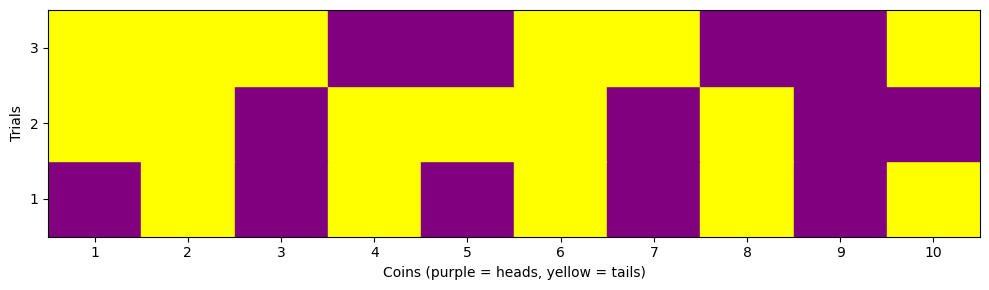
\includegraphics[keepaspectratio,alt={png}]{../images/notes-randomness_notes-randomness_tmp_10_0.png}}
\caption{png}
\end{figure}

\section{Macrostates}\label{macrostates}

To illustrate the macrostates, we will run simulations for 10 coins for
various numbers of flips. Because the number of heads (H) and the number
of tails (T) are equal to 10:

\[H+T = 10\]

It's sufficient to use the number of heads (H) as the macrostate. We can
use this to develop a distribution of the macrostates and thus the
probabilities for different macrostates. We will use the
\texttt{histplot} function from \texttt{seaborn} to plot the
distribution of the macrostates. We wrote a couple functions to simulate
the coin flips and plot the results.

\begin{Shaded}
\begin{Highlighting}[]
\KeywordTok{def}\NormalTok{ simulate\_trials(trials, coins):}
    \CommentTok{\# Simulate flipping coins for each trial}
\NormalTok{    heads }\OperatorTok{=}\NormalTok{ [flip\_coins(coins).count(}\DecValTok{1}\NormalTok{) }\ControlFlowTok{for}\NormalTok{ \_ }\KeywordTok{in} \BuiltInTok{range}\NormalTok{(trials)]}
    \ControlFlowTok{return}\NormalTok{ heads}

\KeywordTok{def}\NormalTok{ plot\_histogram(heads, trials, index, coins):}
    \CommentTok{\# Plot histogram}
\NormalTok{    sns.histplot(heads, }
\NormalTok{                 bins}\OperatorTok{=}\NormalTok{np.arange(coins}\OperatorTok{+}\DecValTok{2}\NormalTok{)}\OperatorTok{{-}}\FloatTok{0.5}\NormalTok{, }
\NormalTok{                 kde}\OperatorTok{=}\VariableTok{False}\NormalTok{, stat}\OperatorTok{=}\StringTok{"density"}\NormalTok{, }
\NormalTok{                 label}\OperatorTok{=}\SpecialStringTok{f\textquotesingle{}}\SpecialCharTok{\{}\NormalTok{trials}\SpecialCharTok{\}}\SpecialStringTok{ Trials\textquotesingle{}}\NormalTok{, }
\NormalTok{                 element}\OperatorTok{=}\StringTok{"step"}\NormalTok{, }
\NormalTok{                 color}\OperatorTok{=}\NormalTok{sns.color\_palette()[index }\OperatorTok{{-}} \DecValTok{1}\NormalTok{],}
\NormalTok{                 alpha}\OperatorTok{=}\FloatTok{0.7}\NormalTok{)}
\NormalTok{    plt.xlabel(}\StringTok{\textquotesingle{}Number of Heads\textquotesingle{}}\NormalTok{)}
\NormalTok{    plt.ylabel(}\StringTok{\textquotesingle{}Frequency\textquotesingle{}}\NormalTok{)}
\NormalTok{    plt.legend()}
\end{Highlighting}
\end{Shaded}

We can see that as we add more trials, the distribution gets more filled
out, and is becoming more symmetric. This distribution looks Gaussian
after a large number of trials. This is the case for a large number of
trials because each event is identical and independent. This is the
\href{https://en.wikipedia.org/wiki/Central_limit_theorem}{central limit
theorem} in action.

\begin{Shaded}
\begin{Highlighting}[]
\CommentTok{\# Set the number of trials and flips}
\NormalTok{trial\_sets }\OperatorTok{=}\NormalTok{ [}\DecValTok{10}\NormalTok{, }\DecValTok{50}\NormalTok{, }\DecValTok{100}\NormalTok{, }\DecValTok{500}\NormalTok{, }\DecValTok{1000}\NormalTok{, }\DecValTok{10000}\NormalTok{]}
\NormalTok{coins }\OperatorTok{=} \DecValTok{10} 

\CommentTok{\# Create a figure and axis}
\NormalTok{plt.figure(figsize}\OperatorTok{=}\NormalTok{(}\DecValTok{12}\NormalTok{, }\DecValTok{8}\NormalTok{))}

\CommentTok{\# Set the seaborn style}
\NormalTok{sns.}\BuiltInTok{set}\NormalTok{(style}\OperatorTok{=}\StringTok{"whitegrid"}\NormalTok{)}

\ControlFlowTok{for}\NormalTok{ trials }\KeywordTok{in}\NormalTok{ trial\_sets:}
    
\NormalTok{    index }\OperatorTok{=}\NormalTok{ trial\_sets.index(trials)}\OperatorTok{+}\DecValTok{1} \CommentTok{\# Set the subplot index}
\NormalTok{    n }\OperatorTok{=} \BuiltInTok{len}\NormalTok{(trial\_sets) }\CommentTok{\# Set the number of subplots}
\NormalTok{    rows }\OperatorTok{=} \BuiltInTok{int}\NormalTok{(np.ceil(n}\OperatorTok{/}\DecValTok{2}\NormalTok{)) }\CommentTok{\# Set the number of rows}
    
\NormalTok{    plt.subplot(}\DecValTok{2}\NormalTok{, rows, index)}
    
\NormalTok{    heads }\OperatorTok{=}\NormalTok{ simulate\_trials(trials, coins)}
\NormalTok{    plot\_histogram(heads, trials, index, coins)}

\NormalTok{plt.tight\_layout()}
\end{Highlighting}
\end{Shaded}

\begin{figure}
\centering
\pandocbounded{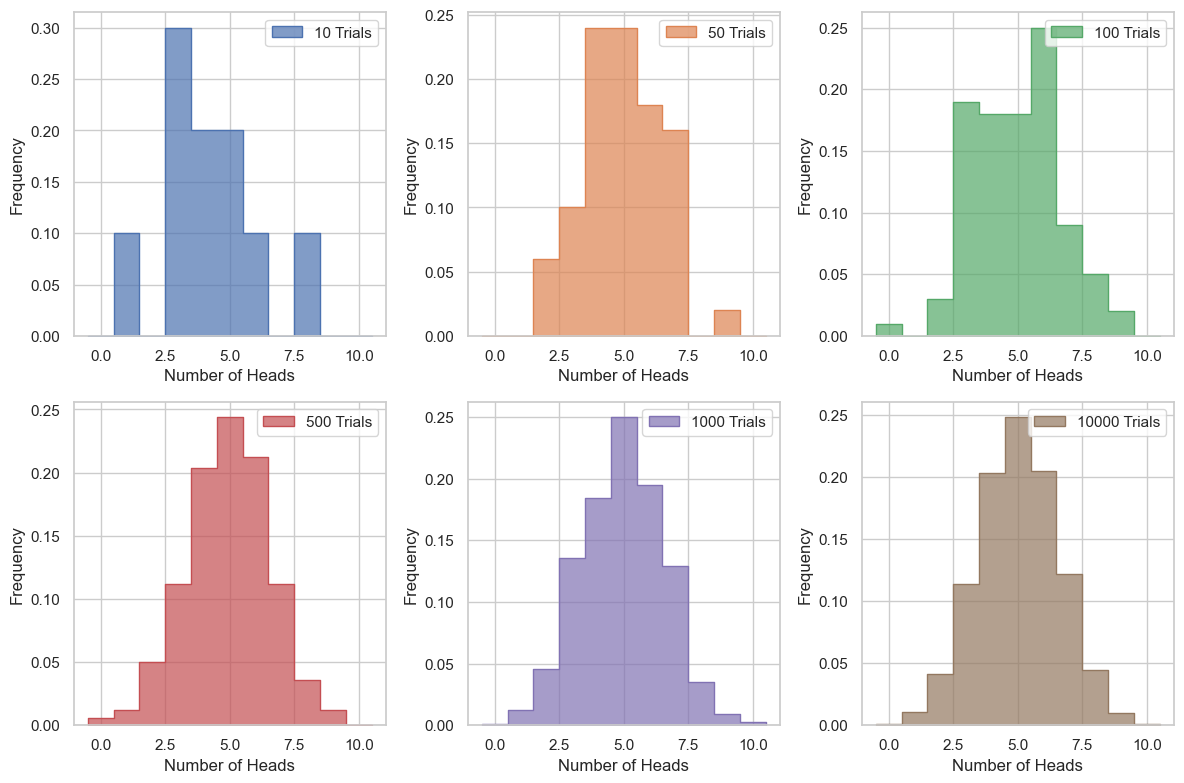
\includegraphics[keepaspectratio,alt={png}]{../images/notes-randomness_notes-randomness_tmp_14_0.png}}
\caption{png}
\end{figure}

This is useful, but the important part of this kind of modeling is to
determine the probablities of the macrostates. We can compute those by
simply determining the number of times a particular macrostate occurs
and dividing by the total number of trials. We wrote two functions to
compute and plot these.

\begin{Shaded}
\begin{Highlighting}[]
\KeywordTok{def}\NormalTok{ calculate\_probabilities(trials, coins):}
    \CommentTok{\# Simulate flipping coins for each trial}
\NormalTok{    heads }\OperatorTok{=}\NormalTok{ [flip\_coins(coins).count(}\DecValTok{1}\NormalTok{) }\ControlFlowTok{for}\NormalTok{ \_ }\KeywordTok{in} \BuiltInTok{range}\NormalTok{(trials)]}
    
    \CommentTok{\# Calculate empirical probabilities}
\NormalTok{    values, counts }\OperatorTok{=}\NormalTok{ np.unique(heads, return\_counts}\OperatorTok{=}\VariableTok{True}\NormalTok{)}
\NormalTok{    probabilities }\OperatorTok{=}\NormalTok{ counts }\OperatorTok{/}\NormalTok{ trials}
    
    \ControlFlowTok{return}\NormalTok{ values, probabilities}

\KeywordTok{def}\NormalTok{ plot\_probabilities(ax, values, probabilities, trials, index):}
    \CommentTok{\# Define marker types}
\NormalTok{    markers }\OperatorTok{=}\NormalTok{ [}\StringTok{\textquotesingle{}o\textquotesingle{}}\NormalTok{, }\StringTok{\textquotesingle{}v\textquotesingle{}}\NormalTok{, }\StringTok{\textquotesingle{}\^{}\textquotesingle{}}\NormalTok{, }\StringTok{\textquotesingle{}\textless{}\textquotesingle{}}\NormalTok{, }\StringTok{\textquotesingle{}\textgreater{}\textquotesingle{}}\NormalTok{, }\StringTok{\textquotesingle{}s\textquotesingle{}}\NormalTok{, }\StringTok{\textquotesingle{}p\textquotesingle{}}\NormalTok{, }\StringTok{\textquotesingle{}*\textquotesingle{}}\NormalTok{, }\StringTok{\textquotesingle{}h\textquotesingle{}}\NormalTok{, }\StringTok{\textquotesingle{}H\textquotesingle{}}\NormalTok{, }\StringTok{\textquotesingle{}D\textquotesingle{}}\NormalTok{, }\StringTok{\textquotesingle{}d\textquotesingle{}}\NormalTok{, }\StringTok{\textquotesingle{}P\textquotesingle{}}\NormalTok{, }\StringTok{\textquotesingle{}X\textquotesingle{}}\NormalTok{]}
    
    \CommentTok{\# Plot empirical probabilities}
\NormalTok{    ax.scatter(values, probabilities, }
\NormalTok{               label}\OperatorTok{=}\SpecialStringTok{f\textquotesingle{}}\SpecialCharTok{\{}\NormalTok{trials}\SpecialCharTok{\}}\SpecialStringTok{ Trials\textquotesingle{}}\NormalTok{, }
\NormalTok{               color}\OperatorTok{=}\NormalTok{sns.color\_palette()[index }\OperatorTok{{-}} \DecValTok{1}\NormalTok{],}
\NormalTok{               marker}\OperatorTok{=}\NormalTok{markers[index }\OperatorTok{\%} \BuiltInTok{len}\NormalTok{(markers)], }\CommentTok{\# Use different marker for each set of trials}
\NormalTok{               s}\OperatorTok{=}\DecValTok{100}\NormalTok{) }\CommentTok{\# Set marker size}
\end{Highlighting}
\end{Shaded}

\begin{Shaded}
\begin{Highlighting}[]
\NormalTok{plt.figure(figsize}\OperatorTok{=}\NormalTok{(}\DecValTok{8}\NormalTok{, }\DecValTok{6}\NormalTok{))}

\CommentTok{\# Set the seaborn style}
\NormalTok{sns.}\BuiltInTok{set}\NormalTok{(style}\OperatorTok{=}\StringTok{"whitegrid"}\NormalTok{)}

\CommentTok{\# Create a single subplot}
\NormalTok{ax }\OperatorTok{=}\NormalTok{ plt.subplot(}\DecValTok{1}\NormalTok{, }\DecValTok{1}\NormalTok{, }\DecValTok{1}\NormalTok{)}

\ControlFlowTok{for}\NormalTok{ trials }\KeywordTok{in}\NormalTok{ trial\_sets:}
    
\NormalTok{    index }\OperatorTok{=}\NormalTok{ trial\_sets.index(trials) }\CommentTok{\# Set the subplot index}
    
\NormalTok{    values, probabilities }\OperatorTok{=}\NormalTok{ calculate\_probabilities(trials, coins)}
\NormalTok{    plot\_probabilities(ax, values, probabilities, trials, index)}

\CommentTok{\# Set x{-}ticks to be centered on the markers}
\NormalTok{ax.set\_xticks(np.arange(}\DecValTok{0}\NormalTok{, coins}\OperatorTok{+}\DecValTok{1}\NormalTok{))}

\NormalTok{plt.xlabel(}\StringTok{\textquotesingle{}Number of Heads\textquotesingle{}}\NormalTok{)}
\NormalTok{plt.ylabel(}\StringTok{\textquotesingle{}Empirical Probability\textquotesingle{}}\NormalTok{)}
\NormalTok{plt.legend()}

\NormalTok{plt.tight\_layout()}
\end{Highlighting}
\end{Shaded}

\begin{figure}
\centering
\pandocbounded{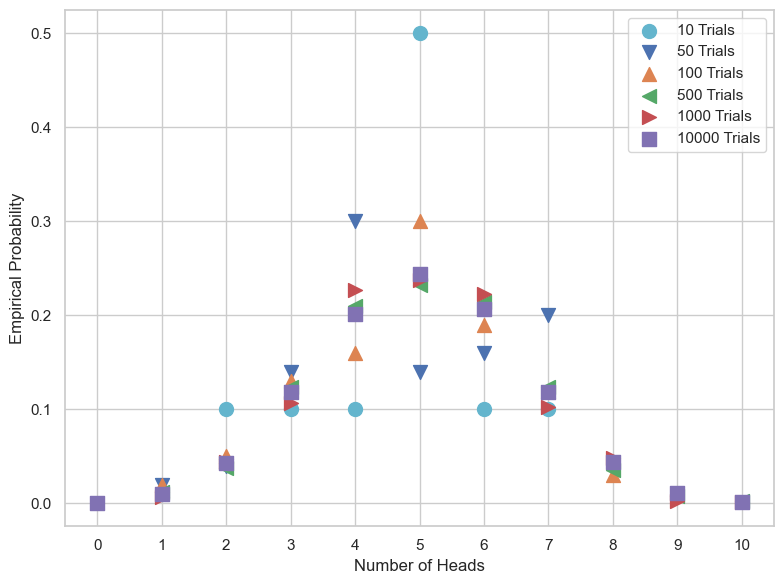
\includegraphics[keepaspectratio,alt={png}]{../images/notes-randomness_notes-randomness_tmp_17_0.png}}
\caption{png}
\end{figure}

It's quite easy to see form here that more trials leads to more stable
and concrete probabilities for each state.

\subsection{Additional Resources}\label{additional-resources}

\subsubsection{Videos}\label{videos}

Here's an interesting application of the models of Poisson process and
Queueing

\href{https://inv.tux.pizza/watch?v=rBIQmwaoZfs}{\pandocbounded{\includegraphics[keepaspectratio,alt={Queuing theory and Poisson process}]{https://markdown-videos-api.jorgenkh.no/youtube/rBIQmwaoZfs?width=720&height=405}}}

\begin{itemize}
\tightlist
\item
  Non-Commercial Link: \url{https://inv.tux.pizza/watch?v=rBIQmwaoZfs}
\item
  Commercial Link: \url{https://youtube.com/watch?v=rBIQmwaoZfs}
\end{itemize}
